\documentclass{article}
\usepackage[T1]{fontenc}
\usepackage{lmodern}
\usepackage{graphicx}
\usepackage{amsmath,amssymb}
\usepackage[a4paper,margin=2cm]{geometry}
\usepackage[absolute,overlay]{textpos}
\setlength{\TPHorizModule}{1mm}
\setlength{\TPVertModule}{1mm}
\usepackage[indonesian]{babel}
\usepackage{hyperref}
\setlength{\emergencystretch}{2em}
% unit: Halaman 29

\begin{document}

% === Halaman 29 (llm) ===

\section*{Transformasi $AddRoundKey()$}

\vspace{95.04mm}

\begin{itemize}
    \item Transformasi ini melakukan operasi XOR antara \textit{round key} dan \textit{state}, dan hasilnya disimpan di \textit{state}.
\end{itemize}

\vspace{10mm}

% deskripsi: Diagram operasi XOR antara matriks 'state' dan 'round key' yang menghasilkan matriks 'state''
% bbox normalisasi: [0.1200, 0.4500, 0.8600, 0.7700]
\begin{textblock*}{155.40mm}(25.20mm,133.65mm)
\noindent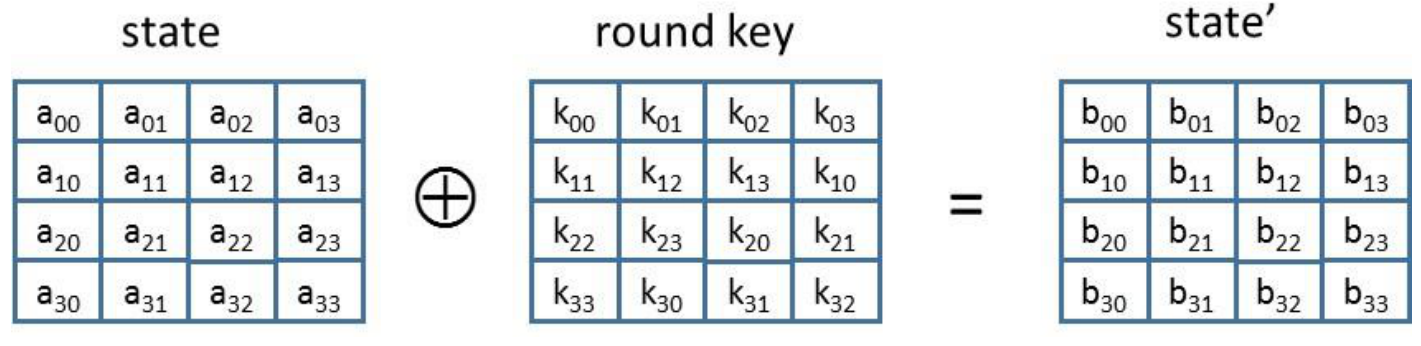
\includegraphics[width=155.40mm,height=95.04mm]{../../images/llm/page_029_img_01.png}%
\end{textblock*}

\end{document}
